\documentclass[12pt]{article}

\usepackage[margin=1in]{geometry}
\usepackage{amsmath,amssymb}
\usepackage{booktabs}
\usepackage{graphicx}
\usepackage{hyperref}
\usepackage{natbib}

\newcommand{\Msun}{M_\odot}
\newcommand{\Mdot}{\dot{M}}
\newcommand{\MdotB}{\dot{M}_B}
\newcommand{\rcoll}{r_{\rm coll}}
\newcommand{\rsonic}{r_{\rm sonic}}
\newcommand{\mfp}{\lambda_{\rm mfp}}
\newcommand{\lcrit}{\ell_{\rm crit}}
\newcommand{\ltyp}{\ell_{\rm typ}}
\newcommand{\feff}{f_{\rm eff}}
\newcommand{\Kn}{\mathrm{Kn}}

\title{Appendix: Self-regulation of the collisionless pile-up\\
       in cooled Bondi accretion onto light PBHs}
\author{M.\ Cantiello}
\date{}

\begin{document}
\maketitle

%----------------------------------------------------------------------
\section{Purpose of this appendix}
\label{app:purpose}

This appendix addresses a possible failure mode of the one-dimensional
Bondi+cooling calculation for very light primordial black holes (PBHs)
embedded in stellar interiors. The concern is that, although the gas is
collisional at the Bondi radius, the flow can become collisionless at
smaller radii. Once this happens, individual particles retain their
thermal transverse velocities and therefore their angular momenta. Since
most of these angular momenta exceed the general-relativistic capture
threshold, most particles miss the black hole on any single pass.

If the entire problem were collisionless, the accretion rate would be set
by the gravitational-capture cross-section rather than by the Bondi
supply. For non-relativistic particles in a Maxwellian bath,
\begin{equation}
  \frac{\Mdot_{\rm coll}}{\MdotB}
  \sim \frac{c_s^2}{c^2}
  \simeq 3\times10^{-6},
  \label{eq:fully_collisionless_scaling}
\end{equation}
which would catastrophically suppress the accretion rate. The central
result of this appendix is that this fully collisionless limit does
\emph{not} apply over the mass range studied in the main paper. The gas
is still collisional at the Bondi radius, so a hydrodynamic supply is
established. The inner collisionless region modifies this supply only
through a moderate pressure feedback.

For the fiducial case $M=10^{-16}\,\Msun$ in the solar core, the final
hydro--kinetic closure gives
\begin{equation}
  \chi \equiv \frac{\Mdot}{\MdotB} \simeq 0.7,
  \label{eq:chi_fiducial_intro}
\end{equation}
corresponding to a $\simeq 30\%$ reduction rather than the factor
$\sim 10^6$ suppression in Eq.~(\ref{eq:fully_collisionless_scaling}).
The correction decreases rapidly with increasing PBH mass and is
negligible by $M\gtrsim10^{-15.5}\,\Msun$.

The physical reason is a self-regulating sequence:
\begin{equation}
  \hbox{missed particles}
  \rightarrow \hbox{cooling and circularization}
  \rightarrow \rho_{\rm pile}\uparrow
  \rightarrow \mfp/r\downarrow
  \rightarrow \hbox{collisionalization}
  \rightarrow \hbox{angular-momentum transport}.
\end{equation}
Thus, in this regime, the PBH is not fed primarily by direct single-pass
loss-cone capture. It is fed by a
recycling/circularization/collisionalization flow whose main effect is to
exert a pressure feedback on the surrounding subsonic Bondi flow.

%----------------------------------------------------------------------
\section{Fiducial scales and ordering of radii}
\label{app:scales}

We consider a PBH of mass $M=10^{-16}\,\Msun$ embedded in the present
solar core, with
$T_\infty=1.57\times10^7\,{\rm K}$,
$\rho_\infty=150\,{\rm g\,cm^{-3}}$,
$\mu=0.85$, and $\gamma=5/3$. The relevant length scales are
\begin{center}
\begin{tabular}{lll}
\toprule
Bondi radius & $r_B=GM/c_{s,\infty}^2$ & $\simeq5\times10^{-6}\,{\rm cm}$ \\
Schwarzschild radius & $r_S=2GM/c^2$ & $\simeq3\times10^{-11}\,{\rm cm}$ \\
Ambient Coulomb mean free path & $\mfp$ & $\sim10^{-7}\,{\rm cm}$ \\
\bottomrule
\end{tabular}
\end{center}
The gas is therefore collisional on the Bondi scale,
$\mfp\ll r_B$. The hydrodynamic supply rate is well defined there.

In the cooled Bondi solution, however, the ratio $\mfp/r$ increases
inward. For the fiducial model, the collisionless transition occurs at
\begin{equation}
  \rcoll \simeq 7000\,r_S \simeq 2\times10^{-7}\,{\rm cm}.
\end{equation}
The flow at this radius is still subsonic, with $\mathcal{M}\simeq0.7$.
The cooling-induced sonic point lies deeper in, at
\begin{equation}
  \rsonic \simeq 600\mbox{--}800\,r_S.
\end{equation}
The ordering for the fiducial case is therefore
\begin{equation}
  r_B > \rcoll > \rsonic > r_S.
\end{equation}
This ordering is crucial. Because $\rcoll$ lies in the subsonic region,
pressure generated by particles returning to the collisional gas can
communicate upstream and modify the Bondi eigenvalue.

\begin{figure}[t]
  \centering
  \IfFileExists{schematic_pileup.pdf}
    {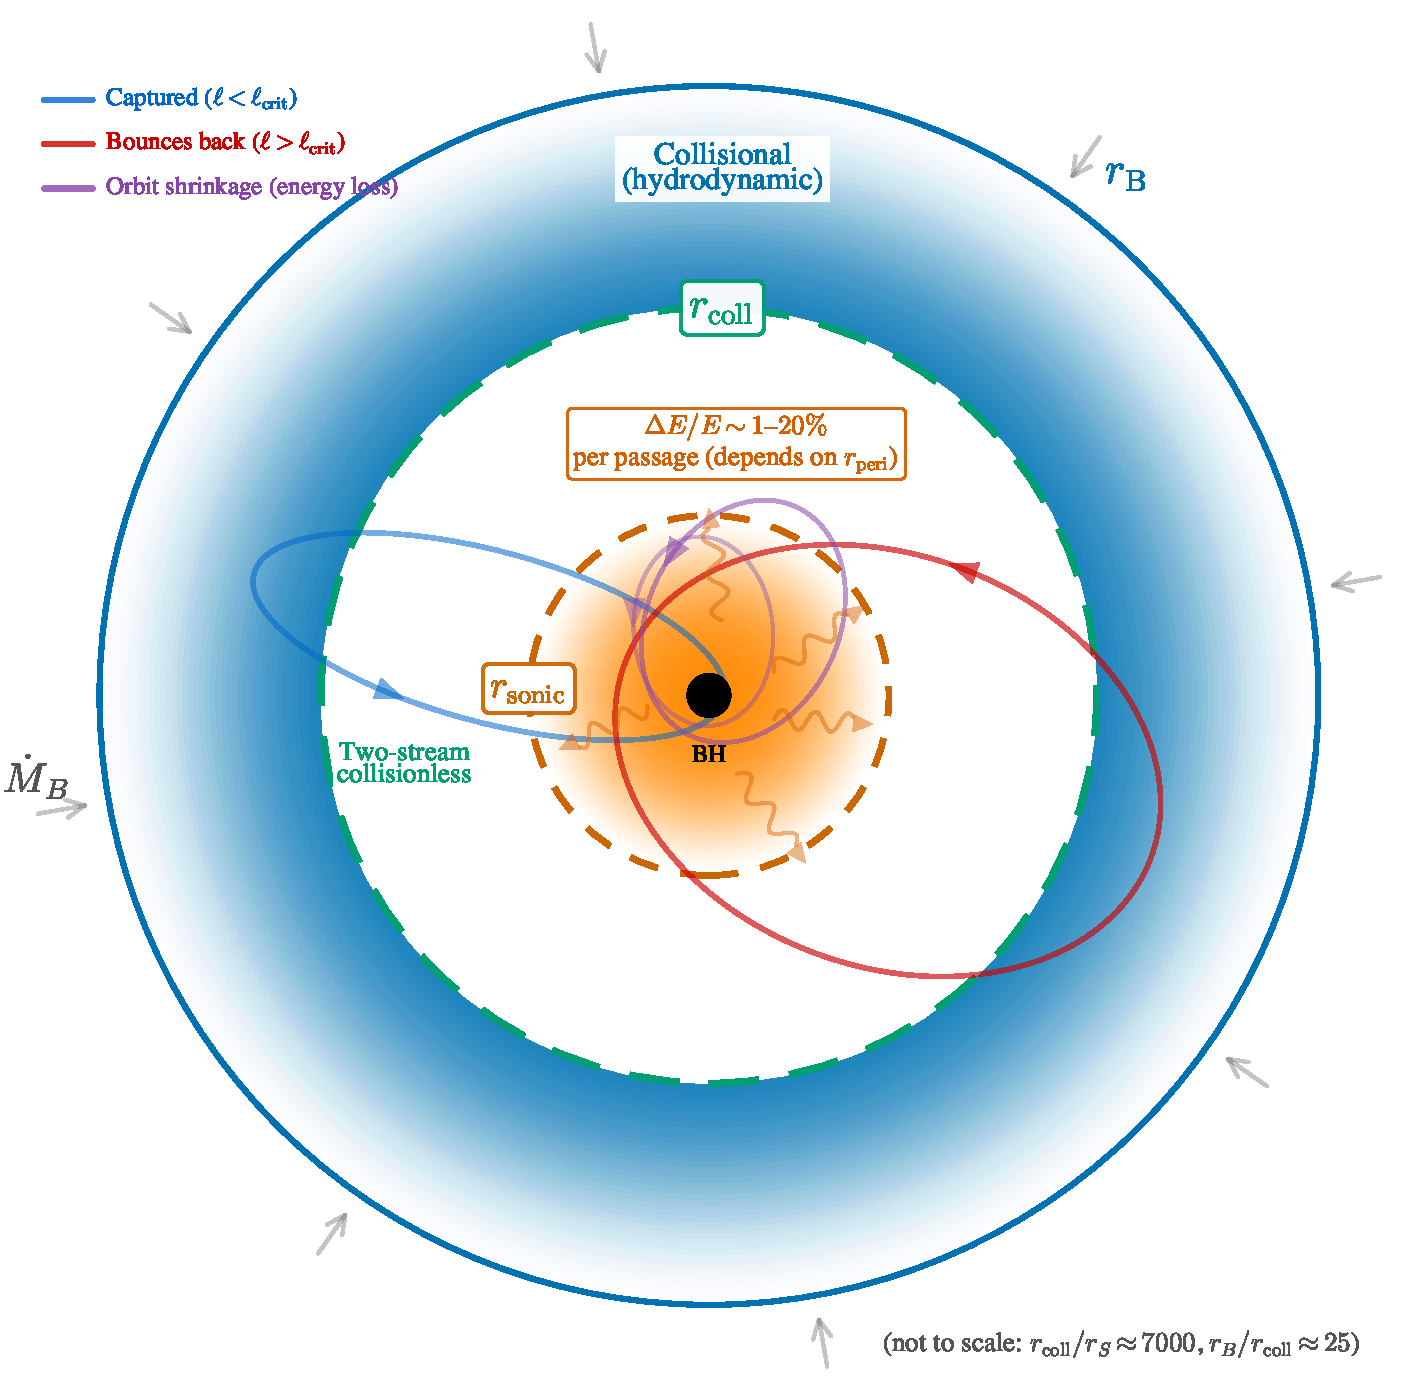
\includegraphics[width=0.86\textwidth]{schematic_pileup.pdf}}
    {\fbox{\parbox{0.8\textwidth}{Schematic figure placeholder:
    schematic\_pileup.pdf}}}
  \caption{Schematic of the collisionless pile-up and recycling process
  (not to scale). The flow is hydrodynamic near $r_B$, becomes
  collisionless below $\rcoll$, and experiences cooling-induced orbit
  shrinkage near the inner region. Direct GR capture occurs only for
  the low-angular-momentum loss cone, $\ell<\ell_{\rm crit}$; most
  particles miss on the first pass and either return to the collisional
  zone or circularize.}
  \label{fig:schematic_rewrite}
\end{figure}

%----------------------------------------------------------------------
\section{Angular momentum barrier and single-pass capture}
\label{app:losscone}

At $\rcoll$, the bulk flow is radial, but individual particles retain
random transverse thermal velocities. With one-component transverse
velocity dispersion
\begin{equation}
  \sigma_\perp = \frac{c_s}{\sqrt{\gamma}},
\end{equation}
the characteristic specific angular momentum is
\begin{equation}
  \ltyp \sim \rcoll\,\sigma_\perp
  \sim 30\,{\rm cm^2\,s^{-1}}.
\end{equation}

A Schwarzschild black hole captures a marginally bound non-relativistic
particle only if its angular momentum is below
\begin{equation}
  \lcrit = \frac{4GM}{c}
  \simeq 1.8\,{\rm cm^2\,s^{-1}}.
\end{equation}
Thus
\begin{equation}
  \frac{\ltyp}{\lcrit}\simeq18.
\end{equation}
Most particles therefore have too much angular momentum to plunge.
Since the transverse velocity is two-dimensional and Rayleigh
distributed, the single-pass loss-cone fraction is
\begin{equation}
  f_{\rm cap}
  \simeq \frac{1}{2}
  \left(\frac{\lcrit}{\ltyp}\right)^2
  \simeq 1.5\times10^{-3}.
  \label{eq:single_pass_capture}
\end{equation}
This small number is the origin of the concern. It would set the
accretion rate in a fully collisionless problem. Here it does not,
because the Bondi-scale gas remains collisional and missed particles can
recycle or circularize rather than being permanently lost.

%----------------------------------------------------------------------
\section{Recycling and the residence-time pile-up}
\label{app:recycling}

Let $\Mdot$ be the hydrodynamic mass flux supplied from the collisional
region outside $\rcoll$, and let $\feff$ be the effective probability
per inward crossing that material is removed from the recycling loop by
direct capture, angular-momentum redistribution, or collisional
transport. In a steady state with such an effective sink,
\begin{equation}
  \Phi_{\rm in}=\frac{\Mdot}{\feff},\qquad
  \Phi_{\rm out}=\frac{1-\feff}{\feff}\,\Mdot,
  \qquad
  \Mdot_{\rm acc}=\feff\Phi_{\rm in}=\Mdot.
  \label{eq:recycling_balance_rewrite}
\end{equation}
The small loss-cone fraction therefore controls the residence time and
density enhancement, not the net supplied flux itself.

The corresponding density enhancement relative to the \emph{current}
inflow is
\begin{equation}
  \xi \equiv \frac{\Phi_{\rm in}+\Phi_{\rm out}}{\Mdot}
  = \frac{2-\feff}{\feff}
  \simeq \frac{2}{\feff}.
  \label{eq:xi_definition_rewrite}
\end{equation}
If orbits were conservative and $\feff=f_{\rm cap}$, this would imply
$\xi\sim10^3$. The pile-up would be enormous. The orbits, however,
are not conservative.

%----------------------------------------------------------------------
\section{Bremsstrahlung limits the residence time}
\label{app:bremsstrahlung}

Particles lose orbital energy through bremsstrahlung during close
encounters. A useful local estimate of the fractional energy loss per
passage at the unperturbed density is
\begin{equation}
  \left(\frac{\Delta E}{E}\right)_0
  \simeq
  \frac{\varepsilon}{\rho}\frac{r}{v}
  \frac{1}{\tfrac12 v^2},
  \label{eq:dEE_local_rewrite}
\end{equation}
where $\varepsilon$ is the bremsstrahlung emissivity. In the cooled
Bondi profiles this gives the representative values
\begin{center}
\begin{tabular}{ccc}
\toprule
$r/r_S$ & $\mathcal{M}$ & $(\Delta E/E)_0$ \\
\midrule
3000 & 0.86 & 1.1\% \\
1000 & 0.96 & 1.3\% \\
550  & 1.08 & 8.0\% \\
300  & 1.33 & 21\% \\
\bottomrule
\end{tabular}
\end{center}
At an enhanced density $\xi\rho$, the cooling rate per unit mass scales
as $\xi$. If a particle makes $N$ passages before its orbit shrinks
substantially, then
\begin{equation}
  N \simeq \frac{1}{\xi(\Delta E/E)_0}.
\end{equation}
Since both inbound and outbound streams contribute to the residence-time
density, $\xi\simeq2N$. Hence
\begin{equation}
  \xi \simeq
  \sqrt{\frac{2}{(\Delta E/E)_0}}
  \simeq 5\mbox{--}13.
  \label{eq:xi_self_limited_rewrite}
\end{equation}
Thus the pile-up self-limits: a larger pile-up increases the cooling
per particle, which shortens the residence time and lowers the pile-up.

This energy loss does \emph{not} imply immediate plunge. To leading
order, bremsstrahlung removes orbital energy more efficiently than
angular momentum. Missed particles therefore shrink and circularize at
approximately
\begin{equation}
  r_{\rm circ}\simeq\frac{\ell^2}{GM},
\end{equation}
rather than falling directly into the PBH. For typical particles,
$\ell\sim\ltyp\simeq18\lcrit$, this is
$r_{\rm circ}\sim10^3$--$10^{3.5}\,r_S$.

%----------------------------------------------------------------------
\section{Orbit-averaged cooling and the fate of missed particles}
\label{app:orbit_averaged}

The single-radius estimate above is useful, but the relevant cooling is
orbit-averaged and depends on angular momentum. We therefore computed
$(\Delta E/E)(\ell)$ by integrating the bremsstrahlung loss along full
Newtonian orbits in the converged cooled background.

The angular-momentum distribution separates into three broad
populations at $\rcoll$:
\begin{center}
\begin{tabular}{llll}
\toprule
Population & Fraction & Angular momentum & Fate \\
\midrule
Direct capture & $\simeq0.2\%$ & $\ell<\lcrit$ & swallowed \\
Reflected & $\simeq33\%$ & $\ell>\ell_{\rm max}$ & rethermalizes near $\rcoll$ \\
Recycling entrants & $\simeq67\%$ & $\lcrit<\ell<\ell_{\rm max}$ & pile-up/circularization \\
\bottomrule
\end{tabular}
\end{center}
For the recycling population,
\begin{equation}
  \left\langle \frac{\Delta E}{E}\right\rangle_{\rm rec}=0.018,
  \qquad
  \langle\xi\rangle_{\rm rec}=11.9.
  \label{eq:orbit_average_results}
\end{equation}
The bulk of the pile-up is therefore controlled by high-$\ell$,
shallow-pericenter particles with modest cooling per orbit,
$(\Delta E/E)\sim1$--$2\%$, rather than by the deeply penetrating
low-$\ell$ tail.

A Markov recycling calculation then follows individual particles
through repeated passages. Because $\langle\xi\rangle\simeq12$, the
number of effective passages is $N\sim\xi/2\sim6$. Combining this with
Eq.~(\ref{eq:single_pass_capture}), the cumulative probability of
direct GR capture before circularization is only of order one percent.
Thus direct capture is not the main sink: most particles circularize.
The essential question becomes whether the circularized material remains
collisionless or self-collisionalizes.

%----------------------------------------------------------------------
\section{Self-induced collisionality of the circularized pile-up}
\label{app:self_collisionality}

The circularized material increases the local density. Since the
Coulomb mean free path scales approximately as $\mfp\propto\rho^{-1}$,
the pile-up lowers the effective Knudsen number. At the circularization
radius,
\begin{equation}
  \Kn_{\rm eff}(\ell)
  = \frac{\Kn_0[r_{\rm circ}(\ell)]}{\xi(\ell)},
  \label{eq:Kneff_rewrite}
\end{equation}
where $\Kn_0=\mfp/r$ is evaluated from the unperturbed cooled profile.
This is an orbit-averaged estimate of the local collisionality. A fully
spatial calculation would compute the pile-up density by binning the
orbital residence time in radius; the estimate above is sufficient for
classifying which angular-momentum bins are clearly collisional,
marginal, or collisionless.

\begin{figure}[t]
  \centering
  \IfFileExists{kn_map.pdf}
    {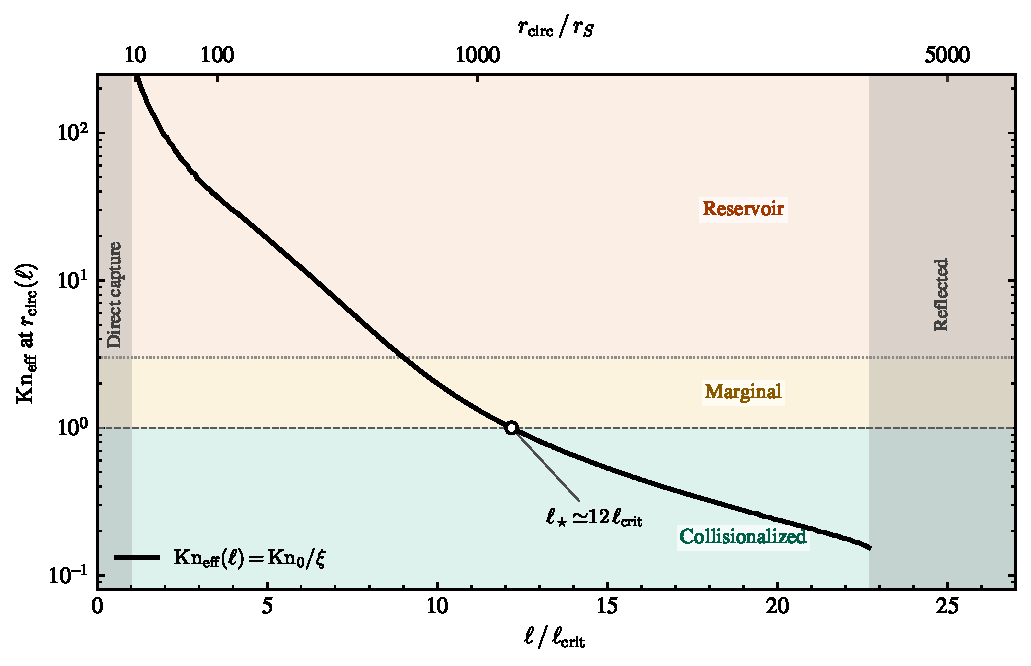
\includegraphics[width=0.86\textwidth]{kn_map.pdf}}
    {\fbox{\parbox{0.8\textwidth}{Knudsen map placeholder:
    kn\_map.pdf}}}
  \caption{Effective Knudsen number at the circularization radius as a
  function of angular momentum. For $\ell\gtrsim12\lcrit$, the
  pile-up-enhanced density makes $\Kn_{\rm eff}<1$, so the
  circularization region is collisional. Only the low-$\ell$ tail
  remains clearly collisionless. The dashed curve gives
  $r_{\rm circ}/r_S$ on the right axis.}
  \label{fig:kn_map_rewrite}
\end{figure}

The result is summarized in Fig.~\ref{fig:kn_map_rewrite}. Among the
non-reflected collisionless entrants,
\begin{itemize}
  \item $\simeq63\%$ circularize in regions with $\Kn_{\rm eff}<1$ and
  are therefore collisionalized by their own pile-up;
  \item $\simeq15\%$ are marginal, with $1<\Kn_{\rm eff}<3$;
  \item $\simeq21\%$ lie in a low-$\ell$ reservoir with
  $\Kn_{\rm eff}>3$.
\end{itemize}
The reservoir is not permanent. The additional mass needed to reduce
$\Kn_{\rm eff}$ to unity in all reservoir bins is only
\begin{equation}
  M_{\rm req}\sim6\times10^{-15}\,{\rm g}.
\end{equation}
Even if supplied only by the reservoir fraction of the reduced inflow,
$\Mdot_{\rm res}\sim f_{\rm res}\chi\MdotB\sim0.08\,{\rm g\,s^{-1}}$,
this mass accumulates in
\begin{equation}
  t_{\rm build}\sim7\times10^{-14}\,{\rm s},
\end{equation}
i.e. on a dynamical timescale. The low-$\ell$ reservoir therefore grows
until it too becomes collisional. This closes the recycling loop:
circularization raises the density, the density lowers the mean free
path, and collisionality restores angular-momentum redistribution and
hydrodynamic inward transport.

%----------------------------------------------------------------------
\section{Hydro--kinetic source coupling and the corrected accretion rate}
\label{sec:stage3b}

The calculations above establish that the collisionless region does
not behave as a simple loss cone. Most particles miss direct GR
capture, lose orbital energy, circularize, and then become marginally
or fully collisional because the pile-up-enhanced density shortens the
mean free path. The remaining question is how this kinetic pile-up
feeds back on the outer hydrodynamic Bondi flow.

The natural representation of this feedback is conservative: the
kinetic region returns fluxes of momentum and energy to the
hydrodynamic flow. We therefore couple the two regions through source
terms derived from the orbit-averaged kinetic model.

\subsection{What the kinetic closure computes}

At a given time, the hydrodynamic solution provides the local state near
the transition region:
\begin{equation}
  \rho(r),\qquad T(r),\qquad v(r),\qquad \Mdot .
\end{equation}
Using this state, the kinetic closure samples the angular-momentum
distribution of particles entering the collisionless region. For each
angular-momentum bin it determines the outcome of the orbit:
\begin{itemize}
  \item direct GR capture, if $\ell < \lcrit$;
  \item reflection and rapid re-thermalization near $\rcoll$, if the
        particle does not enter the collisionless region;
  \item circularization at $r_{\rm circ}(\ell) = \ell^2/(GM)$, followed
        by collisionalization if the pile-up-enhanced Knudsen number is
        below unity or marginal;
  \item temporary reservoir formation for the low-$\ell$ tail, which
        self-collisionalizes after a small additional mass build-up.
\end{itemize}

The closure then assigns a deposition radius to each component. Reflected
particles deposit momentum and energy near $\rcoll$. Circularized and
collisionalized particles deposit them near their circularization radii,
$r_{\rm circ}(\ell)$. The result is a pair of radial source profiles:
a momentum source $S_p(r)$ and an energy source $S_E(r)$.

Physically, $S_p(r)$ is the back-pressure exerted by the thermalizing
pile-up on the inflow, while $S_E(r)$ is the kinetic/orbital energy
deposited into the gas by thermalization. These source terms are
computed from the orbit-averaged kinetic closure; they are not tuned
parameters. For the fiducial $M=10^{-16}\,\Msun$ case, the integrated
momentum feedback corresponds to
\begin{equation}
  \frac{P_{\rm pile}}{P_0} \simeq 5,
\end{equation}
where $P_0$ is the characteristic pressure of the baseline hydrodynamic
solution near the deposition region. The associated thermalization
power is
\begin{equation}
  L_{\rm dep}
  =
  4\pi\int S_E(r)\,r^2\,dr
  \simeq 4\times 10^{17}\ {\rm erg\,s^{-1}} .
\end{equation}

\subsection{How the sources enter the hydrodynamic equations}

The source terms are added directly to the one-dimensional hydrodynamic
equations. We do not add a separate net mass source: the material
represented by the kinetic closure is recycled material drawn from the
same supplied hydrodynamic flux. Its leading effect on the outer
one-dimensional flow is therefore the momentum and energy deposited
during thermalization/collisionalization.

With the sign convention that the inflow velocity is negative ($v<0$),
a positive $S_p$ opposes the infall:
\begin{equation}
  \left.\frac{\partial(\rho v)}{\partial t}\right|_{\rm kin}
  =
  S_p(r),
  \qquad
  S_p>0 \quad \hbox{for outward/back-pressure feedback}.
\end{equation}
The thermalization energy is added to the gas internal-energy equation:
\begin{equation}
  \left.\frac{\partial e}{\partial t}\right|_{\rm kin}
  =
  S_E(r),
\end{equation}
where $e$ is the gas internal-energy density. Here $S_E$ represents
kinetic/orbital energy deposited into the gas by thermalization.
Radiative bremsstrahlung losses are still handled separately by the
cooling term in the energy equation.

In this formulation the kinetic model supplies the momentum and energy
fluxes associated with the pile-up, and the hydrodynamic flow responds
self-consistently; no inner temperature or pressure is prescribed by
hand.

\subsection{Frozen-closure response}

As a first test, we compute $S_p(r)$ and $S_E(r)$ from the baseline
hydrodynamic profile and then hold them fixed while evolving the flow.
We multiply the sources by a dimensionless strength parameter
$\alpha \in [0,1]$,
\begin{equation}
  S_p(r) \rightarrow \alpha S_p(r),
  \qquad
  S_E(r) \rightarrow \alpha S_E(r),
\end{equation}
and ramp $\alpha$ smoothly over $10^4$ hydrodynamic steps. The parameter
$\alpha$ is not physical; it is a numerical diagnostic that lets us
measure how the hydrodynamic solution responds as the kinetic feedback
is gradually turned on.

\begin{table}[h]
\centering
\caption{Frozen-closure response: $\chi = \Mdot/\MdotB$ vs.\ source
  strength $\alpha$ for $M = 10^{-16}\,\Msun$ ($N=1200$, order~1).
  The source profiles are computed from the baseline hydro solution
  and then held fixed.}
\label{tab:alpha}
\begin{tabular}{cc}
\toprule
$\alpha$ & $\chi = \Mdot/\MdotB$ \\
\midrule
0.00 & 1.000 \\
0.10 & 0.959 \\
0.25 & 0.900 \\
0.50 & 0.811 \\
0.75 & 0.735 \\
1.00 & 0.677 \\
\bottomrule
\end{tabular}
\end{table}

The response is smooth and monotonic. No blow-up, shock-like runaway,
or limit cycle appears. At full source strength, $\alpha=1$, the
frozen-closure calculation gives
\begin{equation}
  \chi_{\rm frozen}
  \equiv
  \frac{\Mdot}{\MdotB}
  \simeq 0.68,
  \label{eq:chi_frozen}
\end{equation}
corresponding to a $\simeq 32\%$ reduction relative to the baseline
Bondi value.

\subsection{Self-consistent closure update}

The frozen calculation assumes that the kinetic source profiles remain
equal to their baseline values even after the hydrodynamic flow adjusts.
The final calculation removes this approximation. During the hydro
evolution, we periodically recompute the kinetic closure from the
current hydro state and update the source terms.

Because the kinetic feedback and the subsonic hydro flow respond to
each other, the source terms are updated with under-relaxation. If
$S_p^{(n)}$ and $S_E^{(n)}$ are the source profiles currently being
used by the hydro solver, and $S_{p,{\rm kin}}^{(n)}$ and
$S_{E,{\rm kin}}^{(n)}$ are the newly computed kinetic source profiles
from the current hydro state, we update
\begin{align}
  S_p^{(n+1)}
  &=
  (1-\omega)S_p^{(n)}
  +
  \omega S_{p,{\rm kin}}^{(n)}, \\
  S_E^{(n+1)}
  &=
  (1-\omega)S_E^{(n)}
  +
  \omega S_{E,{\rm kin}}^{(n)} .
\end{align}
Here $\omega$ is a dimensionless under-relaxation parameter. The limit
$\omega=1$ would replace the old source profiles immediately with the
new kinetic prediction. A small value, $\omega\ll1$, makes the feedback
adjust gradually and prevents artificial overshooting. In the fiducial
self-consistent calculation we use
\begin{equation}
  \omega = 10^{-3},
\end{equation}
and recompute the kinetic closure every $1000$ hydrodynamic steps. Thus
the closure changes slowly compared with a single hydro timestep, while
still allowing the kinetic feedback to follow the secular adjustment of
the flow.

\begin{table}[h]
\centering
\caption{Convergence of the self-consistent source-term calculation
  for $M=10^{-16}\,\Msun$. The kinetic source profiles are periodically
  recomputed from the evolving hydro state and updated with
  $\omega=10^{-3}$.}
\label{tab:convergence}
\begin{tabular}{cc}
\toprule
Step & $\chi = \Mdot/\MdotB$ \\
\midrule
80\,000 (end Phase~1) & 1.000 \\
100\,000 & 0.884 \\
120\,000 & 0.749 \\
140\,000 & 0.697 \\
160\,000 & 0.686 \\
200\,000 & 0.686 \\
240\,000 & 0.689 \\
280\,000 & 0.692 \\
\bottomrule
\end{tabular}
\end{table}

The system converges monotonically. The final self-consistent value is
\begin{equation}
  \boxed{
  \chi_{\rm self}
  \equiv
  \frac{\Mdot}{\MdotB}
  \simeq 0.69 .
  }
  \label{eq:chi_self}
\end{equation}
This is very close to the frozen-closure result,
$\chi_{\rm frozen}\simeq0.68$, indicating that the kinetic feedback
strength does not change strongly as the accretion rate is reduced by
$\sim30\%$.

\subsection{Interpretation}

The source-term calculation shows that the kinetic pile-up acts as a
moderate hydrodynamic back-pressure on the subsonic Bondi flow. It does
not shut off the accretion, and it does not produce the fully
collisionless suppression $(c_s/c)^2$. For the fiducial
$M=10^{-16}\,\Msun$ case, the corrected accretion rate is instead
\begin{equation}
  \Mdot \simeq 0.7\,\MdotB .
\end{equation}
The precise numerical value should still be checked at higher
resolution, since the calculation quoted here uses $N=1200$ cells and
order~1 reconstruction. The robust conclusion is that the correction is
moderate, of order tens of percent, rather than catastrophic.

%----------------------------------------------------------------------
\section{Mass dependence}
\label{app:mass_dependence}

The feedback described above matters only when the collisionless
transition lies outside the cooling-induced sonic point,
\begin{equation}
  \rsonic < \rcoll < r_B .
\end{equation}
In this ordering, the pile-up and its thermalization region lie in the
subsonic part of the flow, so the pressure perturbation can communicate
upstream and modify the Bondi eigenvalue. For larger PBH masses,
$\rsonic$ moves outward and overtakes $\rcoll$; the pile-up then lies in
the supersonic region and cannot affect the upstream hydrodynamic
supply.

Applying the self-consistent source-term closure across the lightest
masses gives
\begin{center}
\begin{tabular}{cccc}
\toprule
$\log_{10}(M/\Msun)$ & $\chi=\Mdot/\MdotB$ & reduction & $\rcoll/\rsonic$ \\
\midrule
$-16.0$ & 0.69 & 31\% & 8.9 \\
$-15.8$ & 0.95 & 5\%  & 11.5 \\
$-15.6$ & 0.94 & 6\%  & 0.94 \\
$-15.3$ & 1.00 & 0\%  & 0.06 \\
\bottomrule
\end{tabular}
\end{center}
Thus the correction is sharply localized to the lowest masses in the
paper. Although $\rcoll/\rsonic$ is still large at
$\log_{10}(M/\Msun)=-15.8$, the kinetic source strength and the
associated back-pressure are already much weaker than in the
$10^{-16}\,\Msun$ case, so the correction falls to only a few percent.
For $M\gtrsim10^{-15.5}\,\Msun$, the standard one-dimensional
Bondi+cooling calculation is self-consistent and no pile-up correction
to $\MdotB$ is required.

%----------------------------------------------------------------------
\section{Anomalous collisionality and a conservative lower bound}
\label{app:anomalous}

The kinetic closure used above includes only Coulomb scattering. The
recycling flow at $\rcoll$ is, however, intrinsically counter-streaming:
fresh inflowing material, outbound bouncers, and circularizing matter
coexist in the same volume with substantial relative velocities. Such
configurations are well known to be unstable to current-driven and
Weibel-type plasma microinstabilities, which generate magnetic fields
\emph{de novo} from noise on the electron skin depth.

For the fiducial $M=10^{-16}\,\Msun$ case, the local plasma frequency
gives a skin depth
\begin{equation}
  \delta_e \;=\; c/\omega_p
  \;\sim\; 5\times10^{-8}\,{\rm cm},
\end{equation}
which is already smaller than $\rcoll\sim2\times10^{-7}\,{\rm cm}$.
Self-generated magnetic structures therefore fit comfortably inside
the relevant flow scale. Equipartition with the bulk kinetic energy
would correspond to $B_{\rm eq}\sim4\times10^{8}\,{\rm G}$; even at a
much smaller saturation level $\epsilon_B\sim10^{-6}$, the proton
Larmor radius $r_L\sim10^{-9}\,{\rm cm}$ is already well below
$\rcoll$. The plasma is then magnetized on every scale that matters,
and pitch-angle scattering off the wave field acts as anomalous
collisionality, much as in collisionless shocks.

Anomalous scattering can only \emph{add} to the Coulomb collisionality
already accounted for in Section~\ref{app:self_collisionality}. Its
effects all push $\chi$ towards unity:
\begin{itemize}
\item the low-$\ell$ reservoir bin self-collisionalizes faster, on a
shorter than free-fall timescale;
\item part of the marginal $\Kn_{\rm eff}\sim1$--$3$ population is
moved into the collisional regime;
\item angular-momentum redistribution near $\rcoll$ becomes more
efficient, increasing the effective loss-cone refilling rate.
\end{itemize}
The values $\chi\simeq0.69$ at $10^{-16}\,\Msun$ and the mass scan in
Section~\ref{app:mass_dependence} should therefore be read as a
\emph{conservative lower bound}: pure Coulomb collisions give the
strongest pile-up back-pressure, while any plasma-microinstability
contribution moves the system closer to fully hydrodynamic accretion
at $\MdotB$. A quantitative determination of the saturated
$\epsilon_B$ and of the pitch-angle scattering rate would require a
dedicated kinetic (PIC-level) calculation and is beyond the scope of
this appendix.

%----------------------------------------------------------------------
\section{Fully collisionless limit}
\label{app:fully_collisionless}

The discussion above assumes that the Bondi radius remains collisional,
$r_B\gg\mfp$. For still lower masses, $M\lesssim10^{-18}\,\Msun$,
this fails. The gas is then collisionless already at $r_B$. In that
regime there is no pressure-driven Bondi inflow and no collisional outer
reservoir through which missed particles can recycle. Most ambient
particles undergo ballistic fly-bys; only the GR loss-cone fraction is
captured directly.

Bremsstrahlung losses during close passages may radiatively capture a
small subset of particles into a bound mini-reservoir, and such a
reservoir could self-collisionalize if enough mass accumulates. This
would be a local self-regulation process, but it cannot recreate the
missing hydrodynamic Bondi supply. The time-averaged rate is instead
limited by ballistic and radiative capture from the ambient collisionless
bath,
\begin{equation}
  \Mdot \sim \Mdot_{\rm GR}+\Mdot_{\rm rad.cap.},
  \qquad
  \Mdot_{\rm GR}\sim\frac{c_s^2}{c^2}\MdotB.
\end{equation}
A calculation of $\Mdot_{\rm rad.cap.}$ requires a separate treatment of
radiative capture from a collisionless Maxwellian bath. This regime is
outside the mass range of the present paper.

%----------------------------------------------------------------------
\section{Luminosity and remaining uncertainties}
\label{app:luminosity}

The accretion-rate correction is now reasonably well characterized, but
the luminosity correction is less certain. The physical bremsstrahlung
emissivity in the inner region is controlled by the nonuniform pile-up
density, not by a single global multiplier. The orbit-averaged kinetic
calculation gives $\langle\xi\rangle_{\rm rec}\simeq12$, but this is a
residence-time enhancement rather than a spatially uniform factor. The
density is expected to be concentrated near turning and circularization
radii.

Thus the local emissivity can be substantially enhanced, since
$\varepsilon_{\rm ff}\propto\rho^2$, while the integrated luminosity is
bounded by the orbital energy available along the particle trajectories
and by the reduced accretion rate. A cumulative diagnostic,
\begin{equation}
  L(<r)=4\pi\int_{r_{\rm in}}^r \varepsilon_{\rm ff}(r')r'^2\,dr',
\end{equation}
computed with a regularized orbit-binned density profile, is the next
step needed to turn this into a quantitative luminosity correction. For
now, the radiative efficiency in the lightest models should be regarded
as robust at the order-of-magnitude level, but not yet at the factor-few
level.

%----------------------------------------------------------------------
\section{Summary}
\label{app:summary}

The collisionless inner region does not invalidate the hydrodynamic
Bondi+cooling calculation over the mass range of the paper. The main
points are:
\begin{enumerate}
  \item The gas is collisional at $r_B$ for the masses considered, so a
  hydrodynamic Bondi supply is established.
  \item The flow becomes collisionless only at small radii,
  $\rcoll\sim7000r_S$, where particles retain thermal angular momentum
  and most miss the GR capture cross-section on a single pass.
  \item Bremsstrahlung energy losses limit the residence-time pile-up to
  $\xi\sim5$--$13$, with the orbit-averaged recycling population giving
  $\langle\xi\rangle_{\rm rec}\simeq12$.
  \item Missed particles mainly circularize rather than plunge. The
  resulting pile-up increases the density and lowers the Coulomb mean
  free path, making most of the circularization region collisional.
  \item The remaining low-$\ell$ reservoir requires only a tiny
  additional mass to reach $\Kn\sim1$ and self-eliminates on a dynamical
  timescale.
  \item A conservative hydro--kinetic source coupling gives
  $\chi\equiv\Mdot/\MdotB\simeq0.7$ for $M=10^{-16}\,\Msun$, rising to
  $\chi\simeq0.95$ by $10^{-15.8}\,\Msun$ and $\chi=1$ for
  $M\gtrsim10^{-15.5}\,\Msun$.
  \item Anomalous collisionality from plasma microinstabilities in the
  counter-streaming recycling flow can only add to the Coulomb
  collisionality and push $\chi$ towards unity, so the values above
  should be read as a conservative lower bound.
  \item The fully collisionless $(c_s/c)^2$ suppression applies only
  once $r_B$ itself is collisionless, below the mass range considered
  here.
\end{enumerate}

In short, the PBH is not fed by direct loss-cone capture. It is fed by
a self-regulated recycling/circularization/collisionalization flow. The
main correction is a moderate pressure-feedback reduction of the Bondi
supply at the lowest masses, not a catastrophic collisionless
suppression.

\end{document}